\documentclass[UTF8,10pt,a4paper]{ctexart}
\usepackage[margin=20mm,headheight=26pt]{geometry}
\usepackage{graphicx,xcolor,fancyhdr,booktabs,tabularx,enumitem,hyperref}
\definecolor{ink}{HTML}{12313B}\definecolor{teal}{HTML}{008F89}
\hypersetup{colorlinks=true,urlcolor=teal,linkcolor=teal,pdftitle={WorldGuard 提交材料}}
\setlength{\parindent}{0pt}\setlength{\parskip}{4pt}\linespread{1.12}
\setlist{nosep,leftmargin=1.5em}
\pagestyle{fancy}\fancyhf{}
\fancyhead[L]{\raisebox{-4pt}{
\includegraphics[height=8mm]{assets/logo.png}}\quad\textbf{\textcolor{ink}{WorldGuard}}}
\fancyhead[R]{\small 零界智行\quad U406}
\fancyfoot[L]{\footnotesize 本科生组 · 南京大学 / 东南大学}
\fancyfoot[R]{\footnotesize\thepage}
\renewcommand{\headrulewidth}{0.4pt}
\ctexset{section={format=\Large\bfseries\color{ink},beforeskip=12pt,afterskip=6pt},subsection={format=\large\bfseries\color{teal}}}
\newcommand{\cover}[2]{\vspace*{5mm}{\small\textcolor{teal}{WORLDGUARD / SUBMISSION 2026}}\par\vspace{4mm}{\huge\bfseries\color{ink}#1}\par\vspace{3mm}{\large #2}\par\vspace{4mm}\hrule\vspace{5mm}}
\newcommand{\note}[1]{\par\smallskip\noindent\colorbox{teal!7}{\parbox{0.95\linewidth}{\small #1}}\par\smallskip}
\begin{document}

\cover{正常、边界与失败测试样例}{已保存真实执行输入与结果，可离线复核}
\section{固定条件}
圆盘机器人半径 0.18 m、安全余量 0.05 m、网格分辨率 0.25 m。策略为 strategy\_astar，转弯代价 0.25，净空权重 0。场景、目标和约束见各目录 JSON；不同案例的地图不同，不能混为同条件优劣对照。
\section{正常：01-normal}
来源：A 组 normal。无新增故障的正常基线，验收检查路径足迹与目标是否满足约束。预期：存在安全可行路径时通过并到达。实际：原始验收通过，最终 REACHED。
\section{边界：02-boundary}
来源：B 组 pinch\_clearance\_2。通道收窄后，中心线可能仍可穿过，但机器人足迹所需净空不足。预期：拒绝原始不合格路径，恢复不成功时不授权继续前进。

实际：原始最小剩余净空 $-0.105$ m；恢复未得到合格路径，最终停止（INCONCLUSIVE\_STOP）。不把停止计作到达，也不据此宣称连续空间完全无路。
\section{失败及恢复：03-failure-recovery}
来源：A 组 block\_route\_2。原始规划使用陈旧地图，新增障碍使路径发生足迹冲突。预期：在当前真实地图拒绝原始路径，更新地图后的恢复路径必须再次验收。

实际：原始验收 FAIL，剩余净空 $-0.230$ m；恢复验收 PASS，净空 $0.145$ m，最终到达。原始失败保留。路径长度从 41.5 m 变为 48.0 m，说明恢复存在绕行代价。
\begin{center}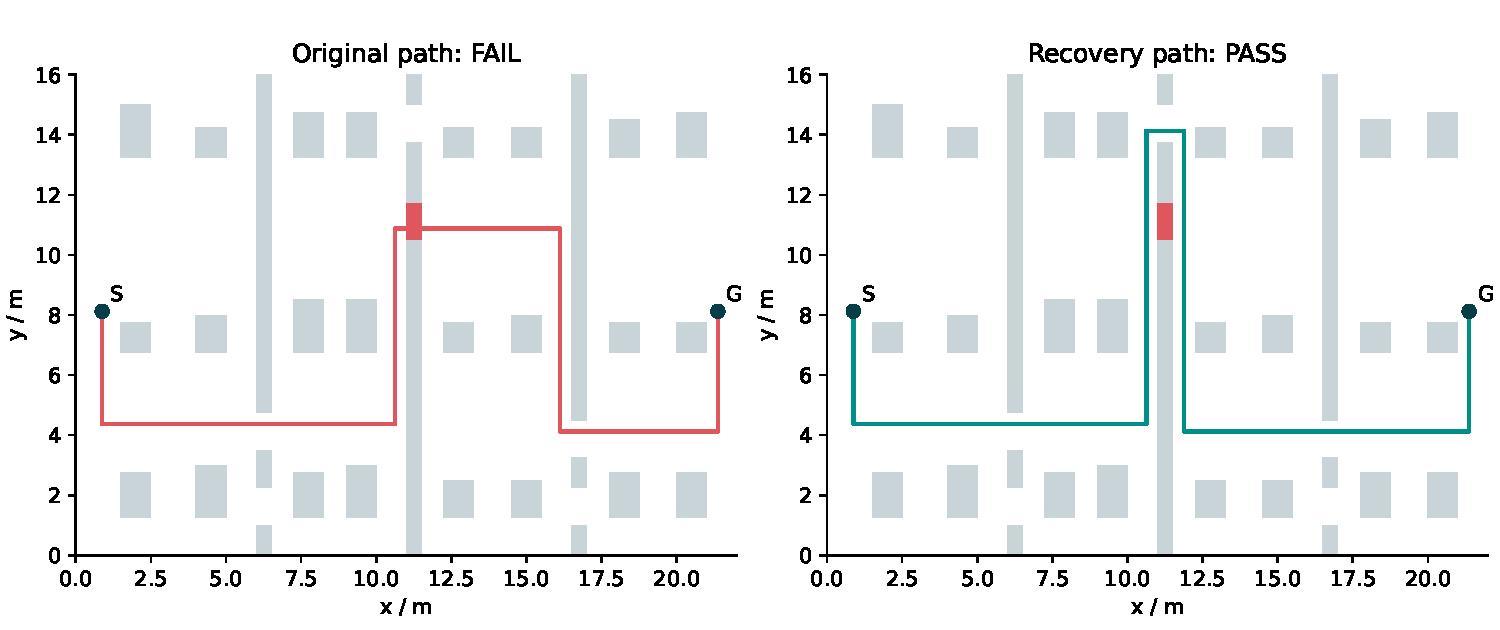
\includegraphics[width=0.85\linewidth]{assets/verified-paths.pdf}\end{center}
\section{复核顺序}
\begin{enumerate}
\item 打开 sample-index.json，确认运行 ID 与案例 ID。
\item 对 manifest 列出的 JSON 按仓库 canonical 规则计算 SHA-256，确认没有改写输入和结果。
\item 按技术指南在新目录运行 CLI replay，比较原始与恢复审计的状态、净空及绑定哈希。
\item 将重放结果和原始 LIVE 记录区分标记；模型决策本身不由几何重放重新证明。
\end{enumerate}
本轮复制时三份样例 manifest 全部匹配。样例是选择性代表案例，不是性能普查或统计优势证明。

\end{document}
